\documentclass[]{article}
\usepackage[makeroom]{cancel}
\usepackage{amsmath}
\usepackage{amsfonts}
\usepackage[margin = 1.1 in]{geometry}
\usepackage{pgfplots}
\usepackage{tikz, bm}
\usetikzlibrary{patterns}
%opening
\title{Focusing Light with a Lens}
\author{Andreas Badea}

\begin{document}
\maketitle
\begin{center}
	\begin{tabular}{l r}
		Date Performed: & March 15, 2018 \\ % Date the experiment was performed
		Instructor: & Dr. Bradley Miller \\ % Instructor/supervisor 
		Partners: & Emilio Folley,\\
		& Mathew Harvey

	\end{tabular}
\end{center}
\section{Introduction}
People generally feel that they have some intuitive understanding of light; they have lived around it their entire lives, vision guiding most all daily activities, but when pressed to describe light most would struggle. For many, light is most commonly thought of as the agent that permits vision. However, this seems a rather anthropocentric perspective. Presumably, there should exist a description of light that exists independent of human observance, and allow one to maintain position of ontological physicalism like any good scientist.

\subsection{A Historical Perspective}
Ancient Greek philosophers explained light not as an agent to aid human vision, but rather as a method by which humans saw. There is a key distinction here. Rather than being a tool for humans, light was a product of humans. Empedocles postulated that there was a small fire in the human eye witch illuminated the world and permitted sight, but he failed to adequately explain why vision was difficult in the dark. Around 300 BC Euclid wrote his treatise on the geometry of vision \textit{Optica}. \footnote{http://photonterrace.net/en/photon/history/} He was troubled by the explanation of light beams streaming from the eyes, noting that one sees the stars immediately after opening one’s eyes, even though stars are very far away. Euclid concluded that light must travel at an infinite speed.


\subsection{Electro-Magnetic Radiation}
In reality light is not made up of beams spouting from one's eyes, rather what we call light is simply a fluctuation in the electric and magnetic fields. Luckily, these fields are governed by a set of relatively simple rules, and we may manipulate these rules to more accurately describe light. Consider the differential forms of Maxwell's equations.

\begin{equation}
\nabla \cdot \mathbf{E} = \frac{\rho}{\epsilon_0}, \ \nabla \cdot \mathbf{B} = 0, \ \nabla \times \mathbf{E} = - \frac{\partial \mathbf{B}}{\partial t}, \ \nabla \times \mathbf{B} = \mu_0 \left( \mathbf{J} + \epsilon_0 \frac{\partial \mathbf{E}}{\partial t} \right)
\end{equation}
Most of the time, light travels in a simple environment: no charges and no currents need be involved. We will simplify things by letting \(  \rho \) and \( \mathbf{J} \) go to zero.
\begin{equation}
\nabla \cdot \mathbf{E} = 0, \ \nabla \cdot \mathbf{B} = 0, \ \nabla \times \mathbf{E} = - \frac{\partial \mathbf{B}}{\partial t}, \ \nabla \times \mathbf{B} = \mu_0 \epsilon_0 \frac{\partial \mathbf{E}}{\partial t}
\end{equation}
If possible, we would like to disentangle \(\mathbf{E}\) and \( \mathbf{B} \). We will do this by taking the curl of both of the curl expressions above. Recall the curl of the curl identity: \(\nabla \times (\nabla \times \mathbf{F}) = \nabla (\nabla \cdot \mathbf{F}) - \nabla^2 \mathbf{F} \). 

\begin{align}
&\nabla \times (\nabla \times \mathbf{E}) = - \nabla \times \left(\frac{\partial \mathbf{B}}{\partial t}\right), \ & \nabla \times (\nabla \times \mathbf{B}) = \nabla \times \left( \mu_0 \epsilon_0 \frac{\partial \mathbf{E}}{\partial t} \right) &
\\
&\nabla \times (\nabla \times \mathbf{E}) = - \frac{\partial }{\partial t} \nabla \times \mathbf{B}, \ &\nabla \times (\nabla \times \mathbf{B}) = \mu_0 \epsilon_0 \frac{\partial }{\partial t} \nabla \times \mathbf{E} &
\\
&\nabla \times (\nabla \times \mathbf{E}) = - \mu_0 \epsilon_0 \frac{\partial^2 \mathbf{E}}{\partial t^2}, \ &\nabla \times (\nabla \times \mathbf{E}) = - \mu_0 \epsilon_0 \frac{\partial^2 \mathbf{B}}{\partial t^2}, &
\\
& \nabla (\nabla \cdot \mathbf{E}) - \nabla^2 \mathbf{E} = - \mu_0 \epsilon_0 \frac{\partial^2 \mathbf{E}}{\partial t^2}, \ & \nabla (\nabla \cdot \mathbf{B}) - \nabla^2 \mathbf{B} = - \mu_0 \epsilon_0 \frac{\partial^2 \mathbf{B}}{\partial t^2}, &
\\
&  \nabla^2 \mathbf{E} = \mu_0 \epsilon_0 \frac{\partial^2 \mathbf{E}}{\partial t^2}, \ &   \nabla^2 \mathbf{B} = \mu_0 \epsilon_0 \frac{\partial^2 \mathbf{B}}{\partial t^2}, &
\end{align}
These final equations effective mean that the local acceleration at a given point is proportional to the local curvature at that same point. This is the same kind of relationship one might see with say, a sheet of rubber. The astute might recognize these as wave equations. This means that, like a rope held taught at two points, one can introduce a perturbation into the electric or magnetic fields and it will propagate forward. Recall that the general wave equation is the form 
\begin{equation}
\nabla^2 \mathbf{F} = \frac{1}{c^2}\frac{\partial^2 \mathbf{F}}{\partial t^2}
\end{equation}
where \(c\) is the wave speed. These imply that both the electric and magnetic fields are waves which propagate forth at a fixed speed : \( 1/\sqrt{\epsilon_0 \mu_0} \), light speed. This demonstrates that light behaves like a wave that will generally move forth at a fixed speed in straight lines.
\begin{figure}[h]
	\caption{Linearly Polarized Light Propagates Forward}
	\centering
	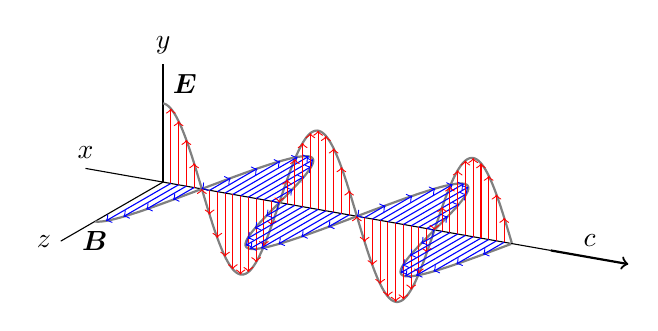
\begin{tikzpicture}[x={(-10:1cm)},y={(90:1cm)},z={(210:1cm)}]
	% Axes
	\draw (-1,0,0) node[above] {$x$} -- (5,0,0);
	\draw (0,0,0) -- (0,1.5,0) node[above] {$y$};
	\draw (0,0,0) -- (0,0,1.5) node[left] {$z$};
	% Propagation
	\draw[->,thick] (5,0,0) -- node[above] {$c$} (6,0,0);
	% Waves
	\draw[gray,thick] plot[domain=0:4.5,samples=200] (\x,{cos(deg(pi*\x))},0);
	\draw[gray,thick] plot[domain=0:4.5,samples=200] (\x,0,{cos(deg(pi*\x))});
	% Arrows
	\foreach \x in {0.1,0.2,...,4.4} {
		\draw[->, red] (\x,0,0) -- (\x,{cos(deg(pi*\x))},0);
		\draw[->, blue] (\x,0,0) -- (\x,0,{cos(deg(pi*\x))});
	}
	% Labels
	\node[above right] at (0,1,0) {$\bm{E}$};
	\node[below] at (0,0,1) {$\bm{B}$};
	\end{tikzpicture}
\end{figure}
\subsection{Passing Through Media}
Taking into account the description of light as a wave propagating forward, it makes sense to conclude that once traveling in a certain direction, light will continue to travel in that straight line. It thus makes sense to describe light as a ray, a straight line emerging from a single point. However, we erred in claiming that the speed of light was constant. We stated that the speed of light was \( 1/\sqrt(\epsilon_0 \mu_0) \), but those constants, the permittivity and permeability of free space respectively, are only truly valid in free space. Light, like electricity and magnetism, need not travel through a vacuum, and the respective constants and wave speeds are different for different media. This shift in speed can mean that a change in media will result in a change in direction. This means that light can appear to bend as it passes through media. This relationship is described by Snell's law.

\begin{figure}[h]
	\caption{Light bends at interface between surfaces with differing speeds of light}
	\centering
	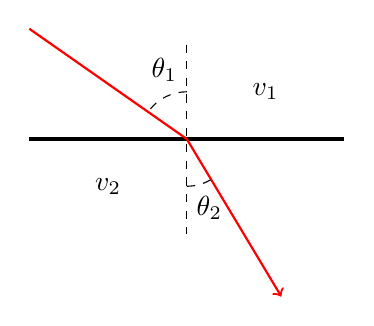
\begin{tikzpicture} [scale = 2]
		\draw [very thick] (-1,0) -- (1,0);
		\draw [thick, red, ->] (-1,0.7) -- (0,0) -- (0.6,-1);
		\draw [dashed,] (0,0.6) -- (0,-0.6);
		\draw [dashed] (0,0.3) node [above left] {\(\theta_1\)} arc (90:145:0.3) ;
		\draw [dashed] (0,-0.3) node [below right] {\(\theta_2\)} arc (270:301:0.3) ;
		\draw (0.5,0.3) node {\(v_1\)};
		\draw (-0.5,-0.3) node {\(v_2\)};
	\end{tikzpicture}
	\hspace{0.5 in}
	\includegraphics[width= 2in]{SAM_0029.jpg}
\end{figure}
When entering a boundary between media at a given angle \(\theta_1\) with respect to the surface normal, a ray of light will exit at an angle \(\theta_2\) such that 
	\begin{equation}
	\frac{\sin(\theta_1)}{\sin(\theta_2)} = \frac{v_2}{v_1}
	\end{equation}
Where \(v_1\) and \(v_2\) are the speeds of light in the respective media. Often we choose to express this relation in terms of refractive indices. A refractive index is a number \(n\) that represents the relative speed of light within a medium. It is defined as the ratio \(c/v\) where \(c\) is the speed of light in a vacuum and \(v\) the speed of light in the medium of interest. This means we may write Snell's law in the form.
\begin{equation}
n_1 \sin(\theta_1) = n_2 \sin(\theta_2) 
\end{equation}
Snell's law follows from Fermat's principle of least time, which states that light travels in the path that will most quickly bring it from one point to another. The algebraic proof of this is beyond the scope of this text\footnote{See Appendix 1}, but a visual explanation is provided in figure 3. Note that the waves of light leaving the source in figure 3 slow down once they enter the medium with a higher optical density, always remaining to the wave front.
\begin{figure}[h]
	\caption{Snell's law}
	\centering
	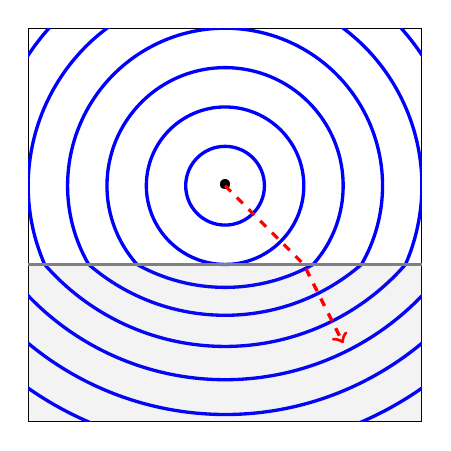
\begin{tikzpicture}[]
	% Axes
	\clip[draw, use as bounding box] (-2.5,-3) -- (2.5,-3) -- (2.5,2) -- (-2.5,2) -- (-2.5,-3);	
	\draw (0,0) node {\textbullet};
		\foreach \r	 in {0.5,1,...,1} {
			\draw [very thick, blue] (0,0) circle (\r);
		}
	\foreach \r	 in {1.5,2,...,5} {
		\draw [very thick, blue] ({-sqrt(\r*\r - 1)},-1) arc ({180+asin(1/\r)}:{-asin(1/\r)}:\r);
		\draw [very thick, blue] ({-sqrt(\r*\r - 1)},-1) arc 
		({180 + asin(2 / (sqrt(\r* \r + 3)))}
		:{360 - asin(2 / (sqrt(\r* \r + 3)))}:
		{sqrt(\r*\r + 3)});
	\fill [gray, opacity = 0.01] (-3,-3) rectangle (3,-1);
}
	\draw [very thick, gray] (-3,-1) -- (3,-1);
	\draw [very thick, red, dashed, ->] (0,0) -- (1,-1) -- (1.5	,-2);

	\end{tikzpicture}
\end{figure}
If light indeed bends when traveling through media, it follows that with strategic positioning of materials we may bend light to our choosing. Most notably this is done with a lens.
\subsection{Lens}
We would like to describe the change in path like undergoes when passing through a lens. We consider a spherical lens of thickness \(d\) and radii \(R_1\) and \(R_2\).
\begin{figure}[h]
	\caption{Lens focusing parallel rays of light}
	\centering
	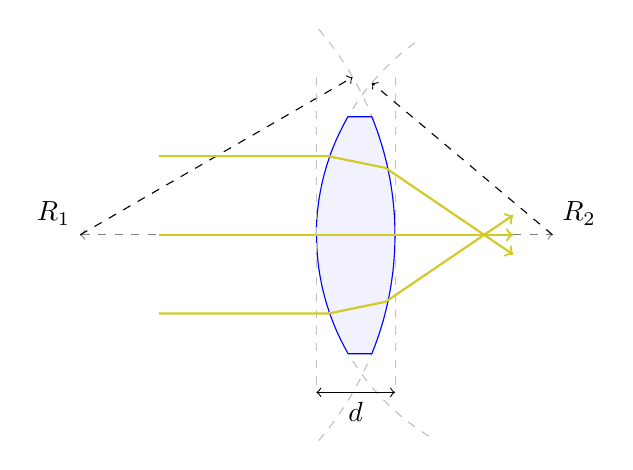
\begin{tikzpicture}
	\draw [gray!50, dashed] (0,0) arc (180:125:3);
	\draw [gray!50, dashed] (0,0) arc (180:240:3);
	\draw [gray!50, dashed] (1,0) arc (0:41:4);
	\draw [gray!50, dashed] (1,0) arc (360:319:4);	
	\draw [blue, fill = blue!05] (0,0) arc (180:150:3) -- (0.705,1.5) arc (22.1:-22.1:4) -- (0.405,-1.51) arc (210:180:3);
	\draw [<->,dashed, gray!!30] (-3,0) -- (3,0);
	\draw [->,dashed] (-3,0) node [above left]{\(R_1\)} -- (0.46,2) ;
	\draw [->,dashed] (3,0) node [above right] {\(R_2\)} -- (0.705,1.93) ;
	\draw [gray!50, dashed] (0,2) -- (0,-2);
	\draw [gray!50, dashed] (1,2) -- (1,-2);
	\draw [<->] (0,-2) -- (0.5,-2) node [below] {\(d\)} -- (1,-2);
	\draw [->, yellow!80!black,thick] (-2,0) -- (2.5,0);
	\draw [->, yellow!80!black,thick] (-2,1) -- (0.15,1) -- (0.88,0.85) -- (2.5,-0.25);
	\draw [->, yellow!80!black,thick] (-2,-1) -- (0.15,-1) -- (0.88,-0.85) -- (2.5,0.25);
	
		\end{tikzpicture}
\end{figure}

Lenses have the property of focusing light. In that, parallel rays of light entering a lens will exit intersecting at a fixed point called the focal point. The distance of this focal point from the lens is called the focal distance, and is a useful way to describe the actions of a lens. We would like to find an expression for this focal distance in terms of the geometry of a lens.

This expression is called the lens makers equation and its derivation is beyond the scope of this text, but gives the power of the lens to be 
\begin{equation}
\frac{1}{f} = \left(n-1\right) \left( \frac{1}{R_1} + \frac{1}{R_2} \right)
\end{equation}
This equation holds both for convergent and divergent lens, as well as concave and convex. Knowing the focal length of a lens allows one to predict the location at which an image will appear. Consider an object placed in front of a thin lens.
\begin{figure}[h]
	\centering
	\caption{Lens Projects Image on Opposite Side}
	\label{FIG:LENS}
	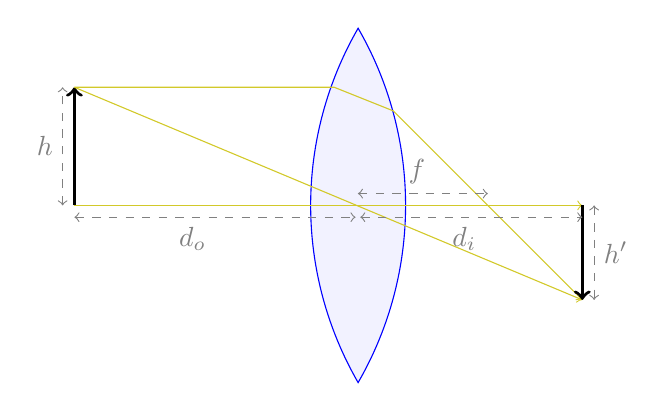
\begin{tikzpicture}[scale = 1.5]
	\draw [->, very thick, black] (-2,0) -- (-2,1);
	\draw [blue, fill = blue!05] (-0,0) arc (180:150:3) arc (30:-30:3) arc (210:180:3);
	\draw [yellow!80!black, ->] (-2,1) -- (0.2,1) -- (0.7,0.8) -- (2.3,-0.8);
	\draw [yellow!80!black, ->] (-2,1) -- (2.3,-0.8);
	\draw [yellow!80!black, ->] (-2,0) -- (2.3,0);
	\draw [->, very thick, black] (2.3,0) -- (2.3,-0.8);
	\draw [<->, gray, dashed] (-2,-0.1) -- (-1,-0.1) node [below] {\(d_o\)} -- (0.38,-0.1);
	\draw [<->, gray, dashed] (0.42,-0.1) -- (1.3,-0.1) node [below] {\(d_i\)} -- (2.3,-0.1);
	\draw [<->, gray, dashed] (-2.1,0) -- (-2.1,0.5) node [left] {\(h\)} -- (-2.1,1);
	\draw [<->, gray, dashed] (2.4,0) -- (2.4,-0.4) node [right] {\(h^\prime \)} -- (2.4,-0.8);
	\draw [<->, gray, dashed] (0.4,0.1) -- (0.9,0.1) node [above] {\(f\)} -- (1.5,0.1);
	\end{tikzpicture}
\end{figure}
We consider 2 rays. One called the chief ray runs through the center of the lens. For thin lenses, this means that it will travel through unmolested in a straight line. The other ray, begins parallel to the optic axis and after exiting passes through the focal point. The figure above clearly illustrates that for thin lenses, two pairs of similar triangles that allow us to set up side ratios. These two are
\begin{equation}
\frac{d_o}{d_i} = \frac{h}{h^\prime}, \text{ and } \frac{h}{h^\prime} = \frac{f}{d_i-f} \label{EQ:3123}
\end{equation}
equating these yields 
\begin{equation}
\frac{d_o}{d_i} = \frac{f}{d_i-f}
\end{equation}
which may be simplified to the rather concise and elegant
\begin{equation}
\frac{1}{f} = \frac{1}{d_o} + \frac{1}{d_i}
\label{EQ:1}
\end{equation}

This equation, paired with measurements of object and image distance allow one to compute the characteristic focal distance of a given lens.
\section{Procedure}
Atop a table lay a large metal rail upon which the optical apparatus rest. A light source, a large lens, and an index card onto which an image shone lay suspended atop this metal rail. The light source lay at the far end of the rail, shining its light across the whole of its span. The light source was a bright bulb kept inside a metal enclosure. One end of  this enclosure was open as to permit the light to shine outward. This opening was covered in a fine metal mesh and a small metal arrow which served as the object to be projected. Further down the rail lay a large glass lens to focus the light,and an index card was placed at the end of the rail. The index card was placed at a point such that projected image, of the metal mesh and small arrow was sharp and in focus. The distance from the source to the lens, the object distance, and the distance from the lens to the projection, the image distance were recorded.

In a final experiment the light source was removed and a nearby window was opened. This light was meant to be the case of light that is arbitrarily far away. The image was focused on a nearby tree.
\section{Data}
The image distance \(d_i\) at which a clear projection of the small arrow and metal mesh was visible was measured at a variety of object distances \(d_o\). The height of the projected object was also measured and recorded. All distances were measured to an accuracy of 0.01 cm.
\begin{figure}[h]
	\caption{Measured Object and Image Distances}
	\centering
\begin{tabular}{|c | c | c ||| c | c| c |}
	\hline
	\(d_0\) (cm) & \(d_i\) (cm) & \(h\) (cm) &  \(d_0\) (cm) & \(d_i\) (cm) & \(h\) (cm)
	\\ \hline
	27.76 & 68.30 & 3.62 & 49.01 & 32.26 & 0.99\\
	29.05 & 60.95 &	3.15 & 51.00 & 31.70 & 1.00 \\
	31.29 &	53.74 &	2.52 & 53.00 & 31.30 & 0.95\\
	32.21 &	48.51 &	2.15 & 54.26 & 30.67 & 0.90 \\
	34.95 &	44.88 &	1.90 & 59.00 & 29.48 & 0.78\\
	37.00 & 41.71 &	1.61 & 64.00 & 28.35 &0.69 \\
	41.00 & 37.20 & 1.36 & LARGE & 19.81 &    \\
    44.00 & 35.03 & 1.25 & LARGE & 19.91 & \\
	46.00 & 33.58 & 1.07 & LARGE & 19.95 & \\ \hline
	
\end{tabular}
\end{figure} 

Characteristics of the environment are to be noted as well.
\begin{figure}[h]
	\centering
	\begin{tabular}{|c|c|}	
		\hline Object height & \(1.55 \pm 0.01\)  cm\\
			\hline Estimated LARGE Distance & \(600 \pm 100\) cm \\ 
				\hline Lens Radii & \(20.4 \pm 0.4\) cm \\ 
					\hline Lens Height & \(7.41 \pm 0.01\) cm \\ 
						\hline Lens Thickness & \(0.78 \pm 0.01\) cm \\
						\hline Lens Top Thickness & \(0.10 \pm 0.01\) cm \\  \hline
						
\end{tabular}
	\end{figure}
\section{Analysis}
Taking the measured object and image distances and computing the focal length of the lens proves incredibly easy. A simple manipulation of equation \eqref{EQ:1} will suffice. 
\begin{equation}
	f = \left( \frac{1}{d_o} + \frac{1}{d_i}\right)^{-1}
\end{equation}
Doing this for all of the measured object and image distances yields 15 separate estimates for the focal distance, all of which are about 19.6 cm. The individual estimates are given below in the order listed above. (top to bottom then left to right) (see figure 7)
\begin{figure}[h]
	\centering
	\caption{Estimates of focal distance of lens}
\begin{tabular}{|c ||| c ||| c |} \hline
	19.74  & 19.61 & 19.55 \\
	19.67  & 19.50 & 19.68 \\
	19.78  & 19.50 & 19.59 \\
	19.36  & 19.41 & 19.66 \\
	19.65  & 19.45 & 19.65 \\ \hline
\end{tabular}
\end{figure}

These figure estimate an average focal distance of 19.59 cm with a sample standard deviation of 0.12 cm.

Another approach to finding the focal distance is to plot the image distance \(d_i\) function of the object distance \(d_o\) and use the focal distance \(f\) as a fitting parameter. This time the alternate equation:

\begin{equation}
d_i = -\frac{f d_o}{f - d_0}
\end{equation}
is used.
\begin{figure}[h]
	\centering
	\caption{Object and Image Distance Compared.}
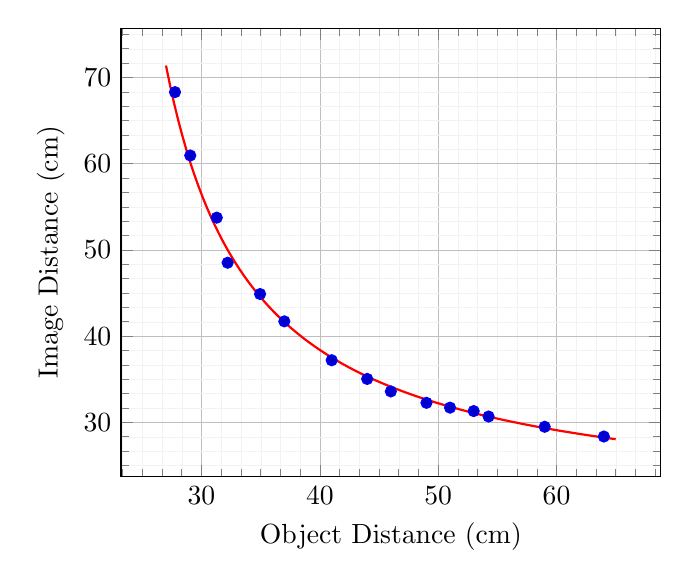
\begin{tikzpicture}
\begin{axis}[xlabel={Object Distance (cm)},
ylabel = {Image Distance (cm)},
grid=both,
minor tick num=5,
grid style={line width=.1pt, draw=gray!10},
major grid style={line width=.2pt,draw=gray!50}]
\addplot+[only marks,
error bars/.cd,
x dir=both,x explicit,
y dir=both,y explicit,
]
table[x=x,y=y]
{
	x      y        y2
27.76	68.3	3.62
29.05	60.95	3.15
31.29	53.74	2.52
32.21	48.51	2.15
34.95	44.88	1.9
37	41.71	1.61
41	37.2	1.36
44	35.03	1.25
46	33.58	1.07
49.01	32.26	0.99
51	31.7	1
53	31.3	0.95
54.26	30.67	0.9
59	29.48	0.78
64	28.35	0.69
};
\addplot[red,samples=111,thick,domain = 27:65] {(-19.59 * x)/(19.59 - x)};
\end{axis}
\end{tikzpicture}
\end{figure}
Doing this yields the somewhat higher but generally similar estimate \(f\) = 19.64 cm. It is also worth noting that the \(R^2\) correlation of the graph above is the incredibly high value of 99.6\%, suggesting that the model for image distance function of object distance is in fact accurate.

This focal distance should extend to the images which used light coming from outside as well as from the window. These were intended to have represented an object that was infinitely far away, and in that case the focal distance should merely be the object distance. However, the object used as a reference for being in focus was a nearby tree, which was, by no fault of its own, not quite infinitely far away. This tree was estimated to have been 6 meters away. Using this estimates for distance yields calculated focal lengths of 19.30, 19.27, 19.21 cm. These are decidedly smaller than other calculated focal distances. Perhaps the tree outside was truly farther than 6 meters away?

\subsection{Error in Focal Lengths}

One might find the error associated with the estimate of the focal distance given the error in each of the measurements. Begin by differentiating the expression for \(f\) with respect to it's two parameters, \(d_i\) and \(d_o\). With a little bit of cleverness one can reduce these derivatives to the convenient expressions :

\begin{equation}
	\frac{\partial f}{\partial d_i} = \frac{f^2}{d_i^2}, \ \ \frac{\partial f}{\partial d_o} = \frac{f^2}{d_o^2}
\end{equation}
These lend themselves to the convenient expression for uncorrelated error
\begin{equation}
	\delta_{f} = f^2 \sqrt{\frac{\delta_{d_o}^2}{d_o^4} + \frac{\delta_{d_i}^2}{d_i^4}}
\end{equation}
However, because the error in measurements for image and object distance are rather small, the overall error in the focal distance is insignificant when compared to the standard deviation of the calculated values.\footnote{Standard deviation uncertainty is about 0.1 cm, uncertainty propagated is typically 0.005 cm}
\subsection{Index of Refraction}
Pairing the lens makers equation with the estimate for focal length above gives a value for the index of refraction of the lens used. Solve the lens maker's equation for index of refraction. Doing this yields the simple, but somewhat clunky expression for index of refraction.

\begin{equation}
n = \frac{f \, R_2 + f \, R_2 + R_1 \, R_2}{f \, R_1 + f \,  R_2}
\end{equation}

However, assuming a symmetrical lens simplifies the expression greatly. Let \(R_1 = R_2 = r\).

\begin{equation}
n = \frac{2\, f + r}{2 \, f}
\end{equation}
or simply,
\begin{equation}
n = 1 + \frac {r}{2 \, f}
\end{equation}
Evaluating this expression with the calculated radius and focal length gives an estimated refractive index of 1.52
\subsection{Uncertainty in Index of Refraction} 
Once again, it is useful to give an estimate of the uncertainty in the calculation for refractive index. Once again take partial derivatives.
\begin{equation}
\frac{\partial n}{\partial f} = -\frac{r}{2 \, f ^2}, \ \ \frac{\partial n}{\partial r} = -\frac{1}{2 \, f},
\end{equation}
These yield the general expression for error.
\begin{equation}
\delta_n = \frac{1}{2 \, f} \sqrt{\frac{\delta_f^2 \, r^2}{f^2} + \delta_r^2}
\end{equation}
This expression gives the uncertainty in the calculation for index of refraction to be 0.01.
\subsection{Magnification}
Recall equation \eqref{EQ:3123}. It stated that the ratio of heights of image to object, the magnification if you will, should have been the same ratio of image distance to object distance.
\begin{equation}
	\frac{d_i}{d_o} = \frac{h^\prime}{h}
\end{equation}

However, this is a bit misleading. Recall that in figure \ref{FIG:LENS} the image is inverted, this means that there is a very real sense in which its height is negative. Taking this into account gives an expression for magnification \(m\).
\begin{equation}
	m = -\frac{d_i}{d_o} = \frac{h^\prime}{h}
\end{equation}

To prove that this relationship holds, one may compare the estimates for magnification using both measured heights, and measured distances.

Doing this for the first few images distances yields a set of relatively similar magnifications. Using the image and object distances gives values -2.46, -2.10, and -1.72 while doing the same with the ratio of heights gives values -2.34, -2.03, -1.63. The values are generally in the same area, as they should be. But there is a non-trivial difference between the two estimates, in fact, the magnification calculated based on height was up to 8\% smaller than that based on distances. On average the magnification calculated using distances was 2\% higher than the one using heights. 
\section{Results and Conclusions}
The focal length of the lens used in the experiment was found to be 19.59 \(\pm\) 0.12 cm, however, this is not particularly easy to compare to any measured physical dimension. Although it does generally agree with the estimate for focal distance with an object that is arbitrarily far away, which was 19.90 when no correction for tree distance was made, and 19.26 using the correction. Interestingly, the 19.59 estimate of the focal length falls nearly exactly in-between the corrected and uncorrected values. It is worth noting that with a large estimate for the 'arbitrarily far away case' the uncertainty in the focal length grows with the object distance, so the uncertainty in the corrected value has a higher uncertainty of about 1 mm. This still places the corrected value out of the range of 19.59 \(\pm\) 0.12 but it explains some variation. The other discrepancy are explained by the difficultly in a accurately focusing on one part of a rather small image. Although, consider that the values for close object distances rely on para-axial approximations, but, being close by, perhaps this is misleading. Aberrant rays will push the focal distance inward, giving a lower effective focal distance than the focal distance for truly para-axial rays. This might mean that the true focal distance is in fact a little bit larger than the calculated 19.59.

The index of refraction calculated is somewhat easier to compare physical values. Recall that it was found to have been \(1.52 \pm 0.01\). This value is a rather sensible index of refraction. For example, it is larger than 1, not implying light travels faster in the medium than in a vacuum. Glass typically has an index of refraction of around 1.5. And the value of 1.52 is closely associated with crown glass \footnote{http://hyperphysics.phy-astr.gsu.edu/hbase/Tables/indrf.html}, the glass most typically used in optical apparatus. This provides strong evidence to conclude that the lens was made of some sort of crown glass.

The magnification calculated by the two methods, by measuring heights and measuring distances, were generally around the same values, however, there was some notable deviation in the two values. This might be explained by the difficulty of accurately measuring the image and object height. The heights were often in awkward positions and the starting place for measuring was often not well defined. This makes accurately measuring the heights difficult and thus makes their respective 
\pagebreak
\section*{Appendix 1 : Proving Snell's Law}
We assume Fermat's principle of least time.

\begin{figure}[h]
	\caption{Light bends at interface between surfaces with differing speeds of light}
	\centering
	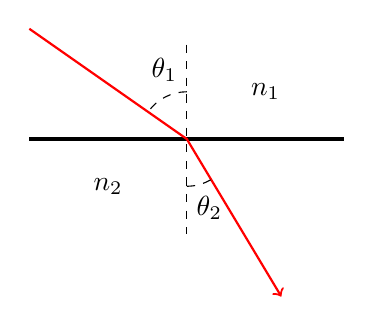
\begin{tikzpicture} [scale = 2]
	\draw [very thick] (-1,0) -- (1,0);
	\draw [thick, red, ->] (-1,0.7) -- (0,0) -- (0.6,-1);
	\draw [dashed,] (0,0.6) -- (0,-0.6);
	\draw [dashed] (0,0.3) node [above left] {\(\theta_1\)} arc (90:145:0.3) ;
	\draw [dashed] (0,-0.3) node [below right] {\(\theta_2\)} arc (270:301:0.3) ;
	\draw (0.5,0.3) node {\(n_1\)};
	\draw (-0.5,-0.3) node {\(n_2\)};
	\end{tikzpicture}
\end{figure}
Without loss of generality, assume that the source point and the terminal point are both 1 vertical unit above and below the interface. Assume that these points are separated horizontally by a distance \(d\). Let the point intersect the interface at a horizontal distance \(x\) from the source point. The time traveled by light is hence 
\begin{equation}
	t = n_1 \sqrt{1 + x^2} + n_2 \sqrt{1+(d-x)^2}
\end{equation}
We take the derivative with respect \(x\) to optimize for minimum time.
\begin{equation}
\frac{\partial t}{\partial x} = {\frac {{ n_1}\,x}{\sqrt {{x}^{2}+1}}}+\,{\frac {{ n_2}\,
		\left( -2\,d+2\,x \right) }{2\sqrt {1+ \left( d-x \right) ^{2}}}}
\end{equation}
The clever might recognize that this may be expressed as
\begin{equation}
\frac{\partial t}{\partial x} = n_1 \sin(\tan^{-1}(x)) - n_2 \sin(\tan^{-1}(d-x))
\end{equation}
Which the geometrically inclined will notice is equivalent to  
\begin{equation}
\frac{\partial t}{\partial x} = n_1 \sin(\theta_1) - n_2 \sin(\theta_2)
\end{equation}
Or minimized at a derivative of zero and equated
\begin{equation}
n_1 \sin(\theta_1) = n_2 \sin(\theta_2)
\end{equation}
Snell's Law!
\pagebreak
\section*{Apendix 2: Lens Maker's Equation}
\begin{figure}[h]
	\centering
	\caption{Lens Projects Image on Opposite Side}
	\label{FIG:LENS}
	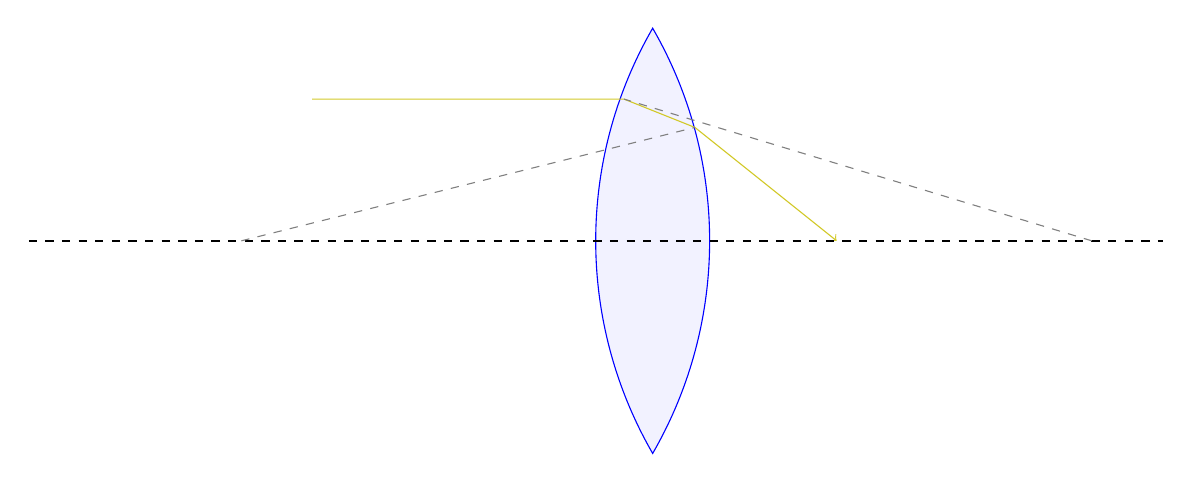
\begin{tikzpicture}[scale = 1.8]
	\draw [blue, fill = blue!05] (-0,0) arc (180:150:3) arc (30:-30:3) arc (210:180:3);
	\draw [yellow!80!black, ->] (-2,1) -- (0.2,1) -- (0.7,0.8) -- (1.7,0);
	\draw [thick,dashed] (-4,0) -- (4,0);
	\draw [gray, dashed] (-2.5,0) -- (0.7,0.8);
	\draw [gray, dashed] (3.5,0) -- (0.2,1);
	\end{tikzpicture}
\end{figure}
We assume angles are small.
\begin{equation}
\theta \approx \sin(\theta) \approx \tan(\theta)
\end{equation}
We use Snell's law to conclude that 
\begin{align}
\sin(\theta_1) = n \sin(\theta_2) \implies \theta_1 = n \theta_2 \\
\sin(\theta_4) = n \sin(\theta_3) \implies \theta_4 = n \theta_3
\end{align}
And then we do some simple trigonometry
\begin{align}
\sin(\theta_1) = \frac{h_1}{R_1} \approx \theta_1 \\
\sin(\theta_5) = \frac{h_2}{R_2} \approx \theta_5 \\
\sin(\theta_6) = \frac{h_2}{f} \approx \theta_6 
\end{align}
We notice the relations between angles
\begin{align}
\theta_7 = \theta_1 - \theta_2 \\
\theta_4 = \theta_5 + \theta_6 \\
\theta_5 = \theta_3 - \theta_7
\end{align}
And finally
\begin{align}
\theta_5 = \theta_3 - \theta_7 = \frac{\theta_4} {n} - (\theta_1 - \theta_2) = \frac{\theta_5 + \theta_6}{2} - \theta_1 + \theta_2 \\
\theta_5 = \frac{\theta_5}{n} +\frac{\theta_6}{n} - \theta_1 + \frac{\theta_1}{n} \implies \frac{h_2}{R_2} = \frac{h_2}{n R_2} + \frac{h_2}{n f} - \frac{h_1}{R_1} + \frac{h_1}{n R_1}
\end{align}
For thin lenses \(h_1 \approx h_2\)
\begin{align}
\frac{n}{h_2} =\frac{1}{R_2} + \frac{1}{f} - \frac{n}{R_1} + \frac{1}{R_1} \implies \frac{1}{f} = \left( n - 1\right) \left( \frac{1}{R_1}  + \frac{1}{R_2}\right)
\end{align}
Lens Maker's Equation!
\end{document}